\documentclass[tikz,border=5pt]{standalone}
\usepackage{pgfplots}
\pgfplotsset{compat=1.18}
\usetikzlibrary{decorations.pathreplacing}
\usepgfplotslibrary{fillbetween}
\usetikzlibrary{arrows.meta}

\definecolor{myCol}{HTML}{A4C7F0}
\definecolor{myCol2}{HTML}{C7F0A4}

\newcommand{\AxisRotator}[1][rotate=0]{%
\tikz[x=0.2cm,y=0.40cm,transform shape,#1]{%
    \draw[line width=0.5px,white,-] 
        (1.7,0.17) -- ++(0.55,0);

    % main arrow
    \draw[line width=0.2ex, -{Latex[length=2mm,width=1.2mm]}] 
        (0,0) arc (-170:170:1 and 1);
}}%

\begin{document}
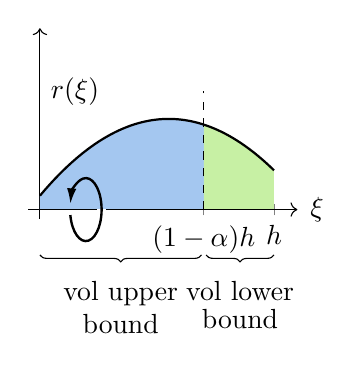
\begin{tikzpicture}
\begin{axis}[
    width=5cm,
    height=4cm,
    axis lines=middle,
    axis line style={->},
    xlabel={$\xi$},
    ylabel={},
    xlabel style={
        at={(axis description cs:0.95,0.05)},
        anchor=west,
        xshift=6pt
    },
    ylabel style={
        at={(axis description cs:0.05,0.95)},
        anchor=south,
        yshift=6pt
    },
    xmin=-0.1, xmax=2.2,
    ymin=-0.1, ymax=2,
    xtick={0,1.4,2},
    xticklabels={$0$,$(1-\alpha)h$,$h$},
    ytick=\empty,
    domain=0:2,
    samples=200,
    clip=false,
    legend style={draw=none, at={(0.02,0.95)}, anchor=west}
]

% Concave function r
\addplot[thick, black, name path=curve]
    {- (x-1.1)^2*0.7 + 1};

\node at (axis cs:0.3,1.3) {$r(\xi)$};

\draw[dashed] (axis cs:1.4,0)  -- (axis cs:1.4,{-(1.4-1.1)^2+1.4});

\draw[
  decorate,
  decoration={brace, mirror}
]
(axis cs:0,-0.5) -- (axis cs:1.38,-0.5)
node[midway, below=6pt] {\shortstack{vol upper\\bound}};

\draw[
  decorate,
  decoration={brace, mirror}
]
(axis cs:1.42,-0.5) -- (axis cs:2,-0.5)
node[midway, below=6pt] {\shortstack{vol lower\\bound}};

\addplot[name path=axis, draw=none] 
    {0};

\addplot[myCol] fill between[
    of=curve and axis,
    soft clip={domain=0:1.4}
];

\addplot[myCol2] fill between[
    of=curve and axis,
    soft clip={domain=1.4:2}
];

\draw (0,0)  -- (2,0)  node [pos=0.2] {\AxisRotator};


\end{axis}
\end{tikzpicture}
\end{document}
